\documentclass[border=5pt]{standalone}
% https://ask.latexstudio.net/ask/question/17933.html
\usepackage{tkz-euclide}
\begin{document}
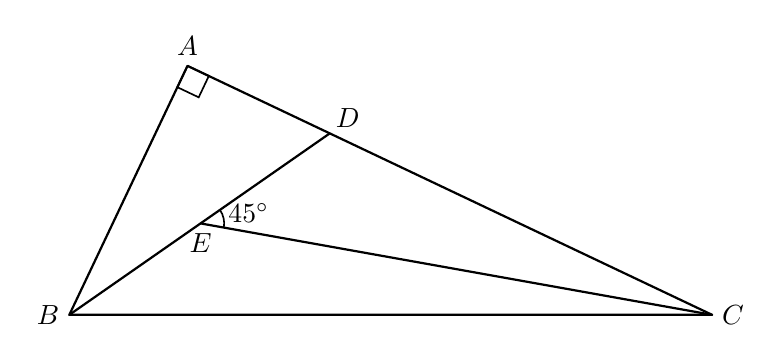
\begin{tikzpicture}[scale=.5]
  \def\c{7}
  \def\b{\fpeval{4+4*sqrt(65)/3}}
  \def\a{\fpeval{sqrt(\c^2+\b^2)}}
  \def\myangle{\fpeval{atan(\b/\c)}}% radians
  \tkzDefPoint(0,0){B}
  \tkzDefPoint(\c*cos(\myangle),\c*sin(\myangle)){A}
  \tkzDefPoint(\a,0){C}
  \tkzDrawPolygon[thick](A,B,C)
  % 取点「D」,满足「AD」=「4/7AB」= 4
  \tkzDefPointWith[linear normed,K=4](A,C) \tkzGetPoint{D}
  % ref: https://ask.latexstudio.net/ask/question/17889.html
  \tkzDrawSegment[thick](B,D)
   % 取点「D」,满足「AD」=「DE」= 4
  \tkzDefPointWith[linear normed,K=4](D,B) \tkzGetPoint{E}
  \tkzDrawSegment[thick](E,C)
    \tkzMarkRightAngle[semithick,size=.6](B,A,C)
    \tkzMarkAngle[semithick,size=.6](C,E,D)
    \tkzLabelAngle[pos=1.25](C,E,D){$45^\circ$}
    \tkzLabelPoint[above](A){$A$}
    \tkzLabelPoint[left](B){$B$}
    \tkzLabelPoint[right](C){$C$}
    \tkzLabelPoint[above right=-2pt](D){$D$}
    \tkzLabelPoint[below](E){$E$}
\end{tikzpicture}
\end{document}